%%%%%%%%%%%%%%%%%%%%%%%%%%%%%%%%%%%%%%%%%%%%%%%%%%%%%%%%%%%%%%%%%%%%%%%%%%%%%%%%%%%%%%%%%%%%%%%
%% Credit: Initial version written by [Ivan C. Christov](http://christov.tmnt-lab.org),      %%
%% Purdue University.                                                                        %%
%% License: GPLv3 (see https://www.gnu.org/licenses/gpl-3.0.en.html)                         %%
%%%%%%%%%%%%%%%%%%%%%%%%%%%%%%%%%%%%%%%%%%%%%%%%%%%%%%%%%%%%%%%%%%%%%%%%%%%%%%%%%%%%%%%%%%%%%%%
\DocumentMetadata
 {
 % testphase = phase-I, % tagging without paragraph tagging
 testphase  = phase-II, % tagging with paragraph tagging
 % testphase  = phase-III, % tagging with paragraph sec, toc, blocks and more
 pdfversion = 2.0, % pdfversion must be set here.
 pdfstandard=ua-2, % pdfstandard can be set too
}
\documentclass[10pt,landscape]{article}

\usepackage[pdftitle={Ideal Flows Handbook}, pdflang=en-US]{hyperref}

\usepackage[tiny]{titlesec}
\titlespacing*{\section}{0pt}{4pt}{8pt}
\usepackage[margin=0.5in]{geometry}
\usepackage{pdflscape}

\usepackage{amsmath,amssymb,amsfonts}

\usepackage{booktabs,makecell}
\usepackage{footnote}
\makesavenoteenv{tabular}

\usepackage{tikz}
\usetikzlibrary{decorations.markings, arrows.meta, bending}
% custom arrow styles for tikz
\tikzset{
  my arrow style/.style={
    >=Stealth[bend],         % arrow tip style
    line width=1.5pt,        % default line thickness
    %arrow style/.style={->} % default arrow type
  }
}
% special arrow styles for ellipses in doublet flow
\tikzset{every path/.style={my arrow style}}
\tikzset{
  ellipsearrow1/.style={
    postaction={
      decorate,
      decoration={
        markings,
        mark=at position 0.26 with {\arrowreversed[my arrow style]{>}}
      }
    }
  }
}
\tikzset{
  ellipsearrow2/.style={
    postaction={
      decorate,
      decoration={
        markings,
        mark=at position -0.1 with {\arrow[my arrow style]{>}}
      }
    }
  }
}
% circled characters with tikz
\newcommand*\circled[1]{\tikz[baseline=(char.base)]{
            \node[shape=circle,draw,inner sep=1pt, line width=0.5pt] (char) {#1};}}

% footnote without a symbol
\makeatletter
\def\blfootnote{\gdef\@thefnmark{}\@footnotetext}
\makeatother

\begin{document}

\thispagestyle{empty}

{\noindent Purdue University, ME 50900 \hfill Prof.\ Ivan C.\ Christov}\\[-2.5mm]
\noindent\makebox[\textwidth]{\rule{\textwidth}{0.5pt}}

\section*{\centering A Brief Handbook of Elementary Ideal Flows\blfootnote{Inspired by Tables 12.1 and 12.2 of Granger's \emph{Fluid Mechanics} (Dover Publications, 2012). Flow \circled{1.}~--~\circled{5.} are the ``building blocks'' and the rest are superposition examples.}}

\noindent
\tagpdfsetup{table/header-rows={1}}%
\resizebox{\textwidth}{!}{%
\begin{tabular}{l @{\qquad} l @{\qquad} l @{\qquad} l @{\qquad} c}
\toprule
\toprule
\thead[l]{\normalsize\textbf{Elementary flow}} & \thead[l]{\normalsize\textbf{Complex potential}, $F = \phi + i \psi$} & \thead[l]{\normalsize\textbf{Potential}, $\phi(x, y)$ or $\phi(r, \theta)$} & \thead[l]{\normalsize\textbf{Streamfunction}, $\psi(x, y)$ or $\psi(r, \theta)$} & \thead[l]{\normalsize\textbf{Sketch of streamlines}} \\
\midrule
\midrule
%%%%%%%%%%%%%%%%%%%%%%%%%%%%%%%%%%%%%%%%%%%%%%%%%%%%%%%%%%%%%%%%%%%%%%%%%%%%%%%%%%%%%%%%%%%%%%%%%
\makecell[l]{\circled{1.} Uniform flow at angle $\alpha$ to the horizontal\\ ~ \\ \phantom{$U$}} & \makecell[l]{$Az$ with $A=Ue^{-i \alpha}$\\ ~ \\ \textcolor{gray}{$U$ is real but $A$ is complex}} & \makecell[l]{$U(x \cos \alpha+ y \sin \alpha)$ \\ ~ \\ {or $U r \cos (\theta-\alpha)$} } & \makecell[l]{$U(y \cos \alpha- x \sin \alpha)$ \\ ~ \\  {or $U r \sin (\theta-\alpha)$} } &
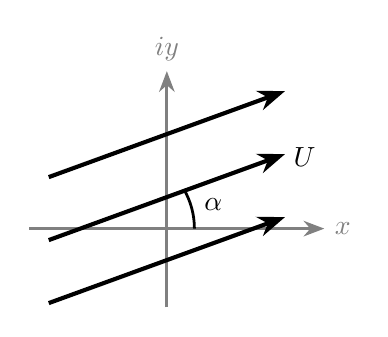
\begin{tikzpicture}[scale=1, baseline=5ex]
    % Axes
    \draw[->, line width=1pt, gray] (-1.75,0) -- (2,0) node[right] {$x$};
    \draw[->, line width=1pt, gray] (0,-1) -- (0,2) node[above] {$iy$};

    % Define angle alpha in degrees
    \def\angle{20}

    % Draw four parallel arrows at angle alpha
    \foreach \y in {-0.4, 0.4, 1.2} {
      \draw[->] (-1.5,{tan(\angle)*(-1.5)+\y}) -- (1.5,{tan(\angle)*1.5+\y});
    }

    % Single U label to the right
    \node at (1.75,{tan(\angle)*2.5}) {$U$};

    % Draw angle arc for denoting alpha
    \draw[-, line width=1pt] (0.35,0) arc[start angle=0, end angle=1.5*\angle, radius=1];
    \node at ({0.6*cos(\angle/2)}, {1.75*sin(\angle/2)}) {$\alpha$};
\end{tikzpicture}
 \\
\midrule
\makecell[l]{\circled{2.} Source ($Q>0$; for sink replace $Q$ by $-Q$) \\ \phantom{\circled{2.}} located at $z_{0}=x_0+iy_0$\\ \phantom{$\frac{Q}{2\pi}$}} & \makecell[l]{$\dfrac{Q}{2 \pi} \log (z-z_0)$\\ ~ \\ \phantom{$\frac{Q}{2\pi}$}} & \makecell[l]{$\dfrac{Q}{2 \pi} \ln \sqrt{(x-x_0)^2+(y-y_0)^2}$\\ ~ \\ \textcolor{gray}{or, for $z_0=0$, $\dfrac{Q}{2 \pi} \ln r$}} & \makecell[l]{$\dfrac{Q}{2 \pi} \tan^{-1}\left(\dfrac{y-y_0}{x-x_0}\right)$ \\ ~ \\  \textcolor{gray}{or, for $z_0=0$, $\dfrac{Q}{2 \pi} \theta$}} &
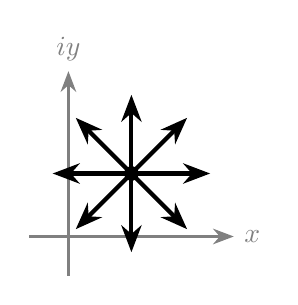
\begin{tikzpicture}[scale=1, baseline=2.75ex]
    % Axes
    \def\ss{0.8}
    \draw[->, line width=1pt, gray] (-1.3,-\ss) -- (1.3,-\ss) node[right] {$x$};
    \draw[->, line width=1pt, gray] (-\ss,-1.3) -- (-\ss,1.3) node[above] {$iy$};

    % Eight rays to represent the source
    \foreach \angle in {0,45,...,315} {
    	\draw[->] (0,0) -- ({cos(\angle)}, {sin(\angle)});
    }
    \filldraw[black] (0,0) circle (2pt);
\end{tikzpicture}
 \\
\midrule
%%%%%%%%%%%%%%%%%%%%%%%%%%%%%%%%%%%%%%%%%%%%%%%%%%%%%%%%%%%%%%%%%%%%%%%%%%%%%%%%%%%%%%%%%%%%%%%%%
\makecell[l]{\circled{3.} Vortex (counterclockwise for $\Gamma >0$)\\ \phantom{\circled{3.}} located at $z_{0}=x_0+iy_0$ \\ \phantom{$\dfrac{\Gamma}{2\pi}$}} & \makecell[l]{$\dfrac{-i \Gamma}{2 \pi} \log (z-z_0)$\\ ~ \\ \phantom{$\dfrac{\Gamma}{2\pi}$}} & \makecell[l]{$\dfrac{\Gamma}{2 \pi} \tan ^{-1}\left(\dfrac{y-y_0}{x-x_0}\right)$\\ ~ \\ \textcolor{gray}{or, for $z_0=0$, $\dfrac{\Gamma}{2 \pi} \theta$}} & \makecell[l]{$-\dfrac{\Gamma}{2 \pi} \ln \sqrt{(x-x_0)^2+(y-y_0)^2}$\\ ~ \\ \textcolor{gray}{or, for $z_0=0$, $-\dfrac{\Gamma}{2 \pi} \ln r$}} &
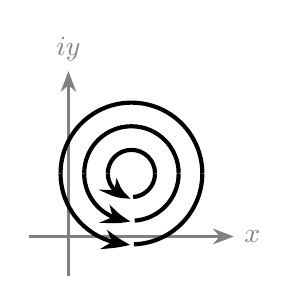
\begin{tikzpicture}[scale=1, baseline=0.75ex]
    % Axes
    \def\ss{0.8}
    \draw[->, line width=1pt, gray] (-1.3,-\ss) -- (1.3,-\ss) node[right] {$x$};
    \draw[->, line width=1pt, gray] (-\ss,-1.3) -- (-\ss,1.3) node[above] {$iy$};

    % Draw 3 concentric circles with breaks
    \draw[line width=1.5pt] (0,0) ++(0.3,0) arc[start angle=0, end angle=180, radius=0.3];
    \draw[->] (0,0) ++(180:0.3) arc[start angle=180, end angle=269, radius=0.3];
	  \draw[line width=1.5pt] (0,0) ++(274:0.3) arc[start angle=274, end angle=360, radius=0.3];
    %
    \draw[line width=1.5pt] (0,0) ++(0.6,0) arc[start angle=0, end angle=180, radius=0.6];
    \draw[->] (0,0) ++(180:0.6) arc[start angle=180, end angle=269, radius=0.6];
	  \draw[line width=1.5pt] (0,0) ++(274:0.6) arc[start angle=274, end angle=360, radius=0.6];
    %
    \draw[line width=1.5pt] (0,0) ++(0.9,0) arc[start angle=0, end angle=180, radius=0.9];
    \draw[->] (0,0) ++(180:0.9) arc[start angle=180, end angle=269, radius=0.9];
	  \draw[line width=1.5pt] (0,0) ++(272:0.9) arc[start angle=272, end angle=360, radius=0.9];
\end{tikzpicture}
 \\
\midrule
%%%%%%%%%%%%%%%%%%%%%%%%%%%%%%%%%%%%%%%%%%%%%%%%%%%%%%%%%%%%%%%%%%%%%%%%%%%%%%%%%%%%%%%%%%%%%%%%%
\makecell[l]{\circled{4.} Doublet located at $z_{0}=x_0+iy_0$\\ \phantom{\circled{4.}} and rotated by angle $\alpha$\\ ~ \\ ~ } & \makecell[l]{$\dfrac{m e^{i \alpha}}{z-z_0}$ \phantom{$\dfrac{m \cos\left(\tan^{-1}\left(\frac{y}{x}\right)\right)}{\sqrt{y^2}}$} \\ ~ \\ \textcolor{gray}{$m$ is real \phantom{$\dfrac{m \cos (\theta - \alpha)}{r}$}}} & \makecell[l]{$\dfrac{m \cos\left(\tan^{-1}\left(\frac{y-y_0}{x-x_0}\right) - \alpha\right)}{\sqrt{(x-x_0)^2+(y-y_0)^2}}$\\ ~ \\ \textcolor{gray}{or, for $z_0=0$, $\dfrac{m \cos (\theta - \alpha)}{r}$}} & \makecell[l]{$-\dfrac{m \sin\left(\tan^{-1}\left(\frac{y-y_0}{x-x_0}\right) - \alpha\right)}{\sqrt{(x-x_0)^2+(y-y_0)^2}}$\\ ~ \\ \textcolor{gray}{or, for $z_0=0$, $-\dfrac{m \sin (\theta - \alpha)}{r}$}} &
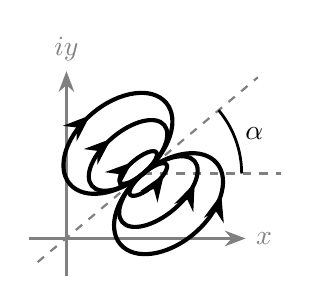
\begin{tikzpicture}[scale=1, baseline=-0.75ex]
    % Axes
    \def\ss{0.825}
    \draw[->, line width=1pt, gray] ({-1.3-0.15},-\ss) -- (1.3,-\ss) node[right] {$x$};
    \draw[->, line width=1pt, gray] ({-\ss-0.15},-1.3) -- ({-\ss-0.15},1.3) node[above] {$iy$};

    % Define angle alpha in degrees
    \def\angle{40}

    % Draw intersecting axes forming angle alpha
    \draw[thick, gray, dashed] (0,0) -- (1.75,0);
    \draw[thick, gray, dashed] ({-1.75*cos(\angle)}, {-1.75*sin(\angle)}) -- ({1.9*cos(\angle)}, {1.9*sin(\angle)});
    % Draw angle arc and label angle
    \draw[-, line width=1pt] (1.25,0) arc[start angle=0, end angle=\angle, radius=1.25];
    \node at ({1.5*cos(\angle/2)}, {1.5*sin(\angle/2)}) {$\alpha$};

    % Draw tilted ellipses tangent at the origin with arrowheads
    \foreach \dy/\a/\b in {-0.1/0.3/0.1, -0.3/0.6/0.3, -0.5/0.8/0.5} {
		\coordinate (C) at ({\dy*sin(\angle)}, {-\dy*cos(\angle)});
        \draw[ellipsearrow1, rotate around={\angle:(0,0)}] (C) ellipse ({\a} and {\b});
    }
    \foreach \dy/\a/\b in {0.1/0.3/0.1, 0.3/0.6/0.3, 0.5/0.8/0.5} {
        \coordinate (C) at ({\dy*sin(\angle)}, {-\dy*cos(\angle)});
        \draw[ellipsearrow2, rotate around={\angle:(0,0)}] (C) ellipse ({\a} and {\b});
    }
\end{tikzpicture}
 \\
\midrule

\makecell[l]{\circled{5.} Flow in a corner of angle $\pi/n$ ($n>1/2$)\\ \phantom{\circled{5.}} $1<n<2$: flows past wedges of angle $2\pi\frac{n-1}{n}$ \\ \phantom{\circled{5.}}  $n=2$: stagnation-point flow onto a horizontal plate} & \makecell[l]{$A z^{n}$\\ ~ \\ \phantom{$U$}} & \makecell[l]{ \textcolor{gray}{[inconventient to use Cartesian coords]} \\ ~ \\ or $U r^n \cos(n\theta)$} & \makecell[l]{ \textcolor{gray}{[inconventient to use Cartesian coords]} \\ ~ \\ or $U r^n \sin(n\theta)$} &
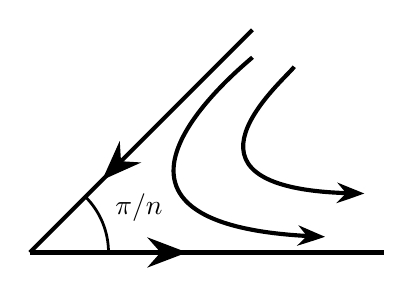
\begin{tikzpicture}[scale=1, baseline=8ex]
    % Define angle
    \def\angle{45}

    % Draw the two rays forming the angle and arrows on each
    \draw[line width=1.5pt] (0,0) -- (4.5,0); % horizontal leg
    \draw[->, line width=2.5pt] (1.7,0) -- (2.0,0);
    \draw[line width=1.5pt] (0,0) -- ({4*cos(\angle)}, {4*sin(\angle)}); % angled leg
    \draw[->, line width=2.5pt] ({1.5*cos(\angle)}, {1.5*sin(\angle)}) -- ({1.3*cos(\angle)}, {1.3*sin(\angle)});

    % Stretched arcs using Bezier curves
    \draw[->] ({4*cos(\angle)}, {4*sin(\angle)-0.35})
      .. controls (2.75,2.4) and (0.1,0.3) .. (3.75,0.2); % outer
    \draw[->] ({4.75*cos(\angle)}, {4.75*sin(\angle)-1})
      .. controls (3.25,2.2) and (1.5,0.75) .. (4.25,0.75); % inner

    % Draw angle arc for denoting the angle pi/n
    \draw[-, line width=1pt] (1,0) arc[start angle=0, end angle=\angle, radius=1];
    \node at ({1.5*cos(\angle/2)}, {1.5*sin(\angle/2)}) {$\pi/n$};
\end{tikzpicture}
  \\
\midrule
\midrule
%%%%%%%%%%%%%%%%%%%%%%%%%%%%%%%%%%%%%%%%%%%%%%%%%%%%%%%%%%%%%%%%%%%%%%%%%%%%%%%%%%%%%%%%%%%%%%%%%
\makecell[l]{\circled{6.} Flow past a Rankine body\\ \phantom{\circled{6.}} ($a$ is a real number/horizontal shift) \\ \qquad $\circled{1}\{\alpha=0\} + \circled{2}\{z_0=-a\} - \circled{2}\{z_0=a\}$ \\ ~ } & \makecell[l]{$U z + \dfrac{Q}{2 \pi} \log\left(\dfrac{z+a}{z-a}\right)$\\ ~ \\ ~ }  & \makecell[l]{$Ux + \dfrac{Q}{2 \pi} \ln\sqrt{\dfrac{(x+a)^2+y^2}{(x-a)^2+y^2}}$\\ ~ \\ \textcolor{gray}{[inconvenient to use polar coords]} } & \makecell[l]{$Uy + \dfrac{Q}{2 \pi}\left[\tan^{-1}\left(\dfrac{y}{x+a}\right)-\tan^{-1}\left(\dfrac{y}{x-a}\right)\right]$ \phantom{$\sqrt{\dfrac{y^2}{y^2}} \hspace{-3em}$}\\ ~ \\ \textcolor{gray}{[inconvenient to use polar coords]} } &
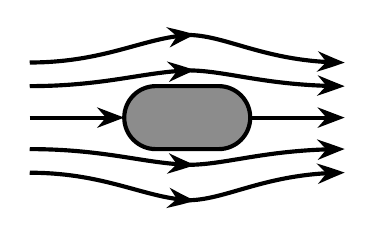
\begin{tikzpicture}[scale=1, baseline=-1.5ex]
    % Draw the object as a pill-shaped, rounded rectangle
    \fill[gray!90, draw=black, rounded corners=0.4cm] (-0.8,-0.4) rectangle (0.8,0.4);

    % Deflected streamlines on the left of the object
    \foreach \y in {-0.7, -0.4, 0.4, 0.7} {
      \draw[->] (-2,\y) .. controls (-1,\y) and (-0.5,1.5*\y) .. (0.1,1.5*\y);
    }

    % Deflected streamlines on the right of the object
    \foreach \y in {-0.7, -0.4, 0.4, 0.7} {
      \draw[->] (0,1.5*\y) .. controls (0.5,1.5*\y) and (1,\y) .. (2,\y);
    }

    % Zero streamline
    \draw[->] (-2,0.0) -- (-0.8,0);
    \draw[->] (0.8,0) -- (2,0);
\end{tikzpicture}
  \\
\midrule
%%%%%%%%%%%%%%%%%%%%%%%%%%%%%%%%%%%%%%%%%%%%%%%%%%%%%%%%%%%%%%%%%%%%%%%%%%%%%%%%%%%%%%%%%%%%%%%%%
\makecell[l]{\circled{7.} Flow past a cylinder with circulation\\ \qquad $\circled{1}\{\alpha=0\} + \circled{4}\{\alpha=0,m=UR^2,z_0=0\}- \circled{3}\{z_0=0\}$ \\ \phantom{$\frac{\Gamma}{2\pi}$} \\ ~ } & \makecell[l]{$U\left(z+\dfrac{R^2}{z}\right) + \dfrac{i\Gamma}{2 \pi} \log z$ \\ ~ \\ ~} & \makecell[l]{$U\left(1+\dfrac{R^2}{x^2+y^2}\right) x - \dfrac{\Gamma}{2 \pi} \tan^{-1}\left(\frac{y}{x}\right)$ \\ ~ \\ $U\left(1+\dfrac{R^2}{r^2}\right) r\cos\theta - \dfrac{\Gamma}{2 \pi} \theta$} & \makecell[l]{$U\left(1-\dfrac{R^2}{x^2+y^2}\right) y + \dfrac{\Gamma}{2 \pi} \ln \sqrt{x^2+y^2}$ \\ ~ \\ $U\left(1-\dfrac{R^2}{r^2}\right) r \sin\theta + \dfrac{\Gamma}{2 \pi} \ln r$} &
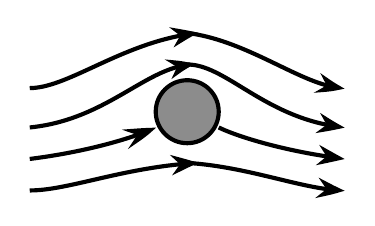
\begin{tikzpicture}[scale=1, baseline=-1.0ex]
    % Draw the circular object with a black border
    \filldraw[fill=gray!90, draw=black] (0,0) circle (0.4);

    % Streamline below the object that enters and exits through it
    \draw[->] (-2,-0.6) .. controls (-1.2,-0.5) and (-0.6,-0.3) .. (-0.4,-0.2);
    \draw[->] (0.4,-0.2) .. controls (0.6,-0.3) and (1.2,-0.5) .. (2,-0.6);

    % Streamlines near the circle (deflected more)
    % left
    \draw[->] (-2,0.3) .. controls (-1.5,0.3) and (-0.8,0.9) .. (0.14,1.0);
    \draw[->] (-2,-0.2) .. controls (-1,-0.1) and (-0.5,0.6) .. (0.1,0.6);
    \draw[->] (-2,-1) .. controls (-1.5,-1) and (-0.8,-0.7) .. (0.14,-0.65);
    % right (mirrored from left)
    \draw[->] (0,1.0) .. controls (0.8,0.9) and (1.5,0.3) .. (2,0.3);
    \draw[->] (0,0.6) .. controls (0.5,0.6) and (1,-0.1) .. (2,-0.2);
    \draw[->] (0,-0.65) .. controls  (0.8,-0.7) and (1.5,-1) .. (2,-1);
\end{tikzpicture}
  \\
\bottomrule
\bottomrule
\end{tabular}
}

%%%% A few examples not ready for public consumption yet

%\begin{tabular}{l @{\qquad} l @{\qquad} l @{\qquad} l @{\qquad} l}
%\midrule
%%%%%%%%%%%%%%%%%%%%%%%%%%%%%%%%%%%%%%%%%%%%%%%%%%%%%%%%%%%%%%%%%%%%%%%%%%%%%%%%%%%%%%%%%%%%%%%%%%
%\makecell[l]{\circled{x.} Flow past a half body \\ \qquad \circled{1} + \circled{2} \\ \phantom{$\frac{Q}{2\pi}$}} & \makecell[l]{$U z + \dfrac{Q}{2 \pi} \log z$\\ ~ \\ \phantom{$\frac{Q}{2\pi}$}}  & \makecell[l]{... \\ ~ \\ ...} & \makecell[l]{... \\ ~ \\ ...} &
%\begin{tikzpicture}[scale=1, baseline=0.75ex]
%    % Draw the left half of the pill-shaped object with a curved cutoff
%    \draw[fill=gray!90, draw=black]
%    (0.4,0.45) -- (-0.4,0.4)
%    arc[start angle=90, end angle=270, radius=0.4cm]
%    -- (0.4,-0.45);
%    %arc[start angle=270, end angle=90, radius=0.4cm];
%
%    % Deflected streamlines on the left of the object
%    \foreach \y in {-0.8, -0.5, 0.5, 0.8} {
%    	\draw[->] (-2,\y) .. controls (-1,\y) and (-0.5,1.5*\y) .. (0.4,1.5*\y);
%    }
%
%    % Zero streamline
%    \draw[->] (-2,0.0) -- (-0.8,0);
%\end{tikzpicture}
%  \\
%\midrule
%%%%%%%%%%%%%%%%%%%%%%%%%%%%%%%%%%%%%%%%%%%%%%%%%%%%%%%%%%%%%%%%%%%%%%%%%%%%%%%%%%%%%%%%%%%%%%%%%%
%\makecell[l]{\circled{x.} Source at the center of a channel \\ ~ \\ ~} & \makecell[l]{$\dfrac{Q}{2 \pi} \ln \sinh (\pi z / a)$ \\ ~ \\ ~ } & \makecell[l]{... \\ ~ \\ ~} & \makecell[l]{... \\ ~ \\ ~} &
%\begin{tikzpicture}[scale=1, baseline=3.5ex]
%	% Draw horizontal reference lines and origin
%    \draw[gray, dashed, line width=1pt] (-0.75,0) -- (2.75,0);
%    \draw[gray, dashed, line width=1pt] (-0.75,1.5) -- (2.75,1.5);
%	   \filldraw[black] (0,0) circle (2pt);
%    % Upper horizontal reference line
%    \draw[->] (-0.5,1.5) -- (2.0,1.5);
%    % Label
%    \node[left] at (-0.2,0.75) {$\dfrac{a}{2}$};
%
%    % Vertical distance marker
%    \draw[<->, line width=0.5pt] (-0.7,0.02) -- (-0.7,1.48);
%
%    % Curved arrows spreading outward
%    \draw[->] (0,0) .. controls (0.2,0.0) and (1,0.0) .. (2.4,0.0);
%    \draw[->] (0,0) .. controls (0.2,0.1) and (1,0.35) .. (2.3,0.35);
%    \draw[->] (0,0) .. controls (0.2,0.5) and (1,0.8) .. (2.2,0.8);
%    \draw[->] (0,0) .. controls (0.2,0.9) and (1,1.25) .. (2.1,1.25);
%\end{tikzpicture}
% \\
%\midrule
%%%%%%%%%%%%%%%%%%%%%%%%%%%%%%%%%%%%%%%%%%%%%%%%%%%%%%%%%%%%%%%%%%%%%%%%%%%%%%%%%%%%%%%%%%%%%%%%%%
%\makecell[l]{\circled{x.} Line vortex near a wall \\ \qquad \circled{3} - \circled{3} \\ ~ } & \makecell[l]{$\dfrac{i \Gamma}{2 \pi} \ln \left(\dfrac{z+a}{z-a}\right)$ \\ ~ \\ ~} & \makecell[l]{... \\ ~ \\ ~} & \makecell[l]{... \\ ~ \\ ~} &
%\begin{tikzpicture}[scale=1, baseline=-0.75ex]
%    % Draw the rectangular bar
%    \fill[gray!90] (-1.5,0.5) rectangle (1.5,0.7);
%    \draw[] (-1.5,0.5) rectangle (1.5,0.7);
%
%    % Curved arrow to the left between bar and circles
%    \draw[->] (1.4,-0.15) to[out=145, in=35] (-1.5,-0.15);
%
%    % Two concentric counterclockwise circular arrows
%    \draw[->] (0,-0.6) arc[start angle=270, end angle=630, radius=0.25];
%    \draw[->] (0,-0.85) arc[start angle=270, end angle=630, radius=0.5];
%\end{tikzpicture}
% \\
%\midrule
%\end{tabular}

\end{document}
